
\chapter{Integración}

En este capítulo vamos a ver como funciona el sitema de integración. Para ello explicaremos en detalle cada uno de los componentes del sistema.\\

Si nos fijamos en la Figura \ref{fig:general_diagram} podemos ver como la \iface{} actúa como puente entre \hs{} y \wday{}. 

\begin{figure}[H]
\centering

    
\pagestyle{empty}
\begin{tikzpicture}
  \path[mindmap,concept color=black,text=white]
    node[concept] {\Large \textbf{Interfaz}}
    [clockwise from=120]
    child[concept color=orange, text=black] {
      node[concept] {App HubSpot}
      [clockwise from=90, inner sep=0.1cm]
      child { node[concept] {\textbf{HubSpot}} }
    }
	child[concept color=blue!35!cyan, text=black] {
      node[concept] {\textbf{Workday}}
    }
    ;
\end{tikzpicture}



\caption{Diagrama general del sistema \protect\footnotemark{}} 
\label{fig:general_diagram}
\end{figure}

\footnotetext{Modificación del ejemplo de \href{http://www.texample.net/tikz/examples/computer-science-mindmap/}{\textit{Till Tantau}}}	

Explicaremos como funcionan \hs{} y \wday{}. Como están organizados y cual es su estructura. También explicaremos los métodos de integración con los que cuenta cada una de las aplicaciones.
Por último, explicaremos en detalle el diseño de la \iface{} así como sus características.\\

La \iface{} esta conectada tanto a \hs{} como a \wday. 

A \hs{} se conecta a través de una aplicación que necesitamos crear en \hs{} y la comunicación  puede ser bidireccional. De la \iface{} hacia \hs{} se hace mediante peticiones \acrshort{http} a la \acrshort{api} de \hs{}. 
La comunicación en la otra dirección se realiza mediante los webhooks declarados en la aplicación de \hs{}\\

Por otro lado está \wday{} cuya comunicación es unidireccional. Únicamente existe comunicación propiamente dicha de la \iface{} hacia \wday. \wday{} sí que responde a algunas peticiones \acrshort{http} con información, pero nunca inicia un mensaje hacia la \iface.

\section{\hs{}}
En esta sección vamos a describir toda la información que necesitamos saber sobre \hs{} para entender la Integración.

%El \acrshort{crm} \hs{} permite realizar integraciones gracias a su \acrshort{api} \acrshort{rest}.
Primero debemos tener en cuenta que \hs{} se encuentra organizado en objetos. Y toda la información almacenada en \hs{} pertenece a uno de los siguientes tipos de objetos:

\begin{itemize}
	\item \textit{Contacts} o Contacto
	\item \textit{Companies} o Compañía
	\item \textit{Deals} u Oportunidad
\end{itemize}

Cada objeto tiene una serie de propiedades por defecto a las que se pueden añadir propiedades personalizadas.
Es importante tener en cuenta las relaciones posibles entre los distintos tipos de objetos.

\begin{itemize}
	\item \textit{Contacts}
	\begin{itemize}
		\item Un contacto puede ser asociado con un único objeto compañía.
		\item Un contacto puede ser asociado con múltiples objetos oportunidad.
	\end{itemize}
	\item \textit{Companies}
	\begin{itemize}
		\item Una compañía puede estar asociada a múltiples contactos.
		\item Una compañía puede estar asociada a múltiples oportunidades.
	\end{itemize}
	\item \textit{Deals}
	\begin{itemize}
		\item Un \textit{deal} puede estar asociado a múltiples objetos contacto y a múltiples objeto compañía.
	\end{itemize}
\end{itemize}

En \hs{} un \textit{deal} puede estar asociado a una o más \textit{companies}. Para el caso de nuestra integración a lo sumo habrá un \textit{company} asociado a cada \textit{deal}.

Los objetos que nos interesan para nuestra integración son \textit{deal} y su \textit{company} asociado. La creación o modificación de un \textit{deal} iniciaran procesos de integración.



\subsection{Descripción del objeto \textit{Deal}}
	Es un objeto de \hs{} que representa una oportunidad de negocio con cierto cliente. Por defecto en \hs{} tenemos las siguientes propiedades asociadas a un deal:			
		\textit{Deal Id}, \textit{Amount}, \textit{Close Date}, \textit{Closed Lost Reason}, \textit{Closed Won Reason}, \textit{Create Date}, \textit{Deal Description}, \textit{Deal Name}, \textit{Deal Stage}, \textit{Deal Type}, \textit{Hubspot Owner}, \textit{Last Activity Date}, \textit{Last Modified Date}, \textit{Number of Contacts},
		\textit{Opp number}, \textit{Owner Assigned Date}, \textit{Pipeline}.
		
		Adicionalmente en la empresa se han creado propiedades personalizadas: \textit{Practice}, \textit{Transaction Amount}, \textit{Transaction Currency}.\\
		
		Las propiedades más importantes a tener en cuenta en la integración son las siguientes:
		\begin{itemize}
			\item \textbf{Deal id}: Identificador unívoco del \textit{deal} de \hs.
			\item \textbf{Close date}: Se trata de la fecha en la que se ha cerrado el acuerdo.
			\item \textbf{Deal Description}: Información describiendo el \textit{deal}.
			\item \textbf{Deal name}: Nombre del \textit{deal}.
			\item \textbf{Deal Stage}: estado en el que se encuentra el \textit{deal}. Esta se trata de una de las propiedades más importantes. 
				Esta propiedad puede tomar los siguientes valores.
				\begin{itemize}
					\item[$\circ$] Appointment Scheduled: Cuando se ha fijado una cita con el cliente.
					\item[$\circ$] Initial Contact: Si ya se ha tenido un primer contacto con el cliente.
					\item[$\circ$] Opportunity Identfied: En caso de que se haya identificado una oportunidad de negocio con el cliente.
					\item[$\circ$] Preparing Proporsal: Si se está preparando una proposición de oferta al cliente.
					\item[$\circ$] Proporsal Sent: Una vez se haya enviado la proposición de oferta al cliente.
					\item[$\circ$] Decision Maker Bought In: Una vez la oferta ya esta hecha y el cliente tiene la posibilidad de decidir si la acepta o no.
					\item[$\circ$] Contract Sent: Cuando el contrato se ha enviado al cliente.
					\item[$\circ$] Closed Won: Si la oportunidad de negocio se ha cerrado favorablemente.
					\item[$\circ$] Closed Lost: En caso de que se haya perdido la oportunidad con el cliente.
				\end{itemize}
		\end{itemize}
		
		
		Es de especial importancia la propiedad \textit{Deal Stage}, ya que dependiendo de su valor se realizará o no la sincronización.
		La propiedad \textit{Deal Stage} representa el estado en el que se encuentra un \textit{deal}.
		
		
		\begin{figure}[H]
\centering
\begin{tikzpicture}[
	scale=0.75,
	start chain=1 going below, 
	node distance=1mm,
	stage/.style={
		scale=0.75,
		on chain=1,
		rectangle,
		rounded corners,
		draw=black, 
		very thick,
		text centered,
		text width=8cm,
		minimum height=12mm
		},
	discovery/.style={
		fill=cyan!30
	},
	progress/.style={
		fill=blue!30
	},
	closure/.style={
		fill=green!30
	},
	phase/.style={
		scale=0.75,
		on chain=1,
		minimum height=12mm,
		text width=2cm,
		text centered
	},
	every node/.style={font=\sffamily}
]



% Discovery phase
\node [stage, discovery] (AS) {Appointment Scheduled};
\node [stage, discovery, continue chain=going below] (IC) {Initial Contact};
% Progress phase
\node [stage, progress] (OI) {Opportunity Identfied};
\node [stage, progress] (PP) {Preparing Proporsal};
\node [stage, progress] (PS) {Proporsal Sent};
\node [stage, progress] (DM) {Decision Maker Bought In};
\node [stage, progress] (CS) {Contract Sent};
% Closure phase
\node [stage, closure] (CW) {Closed Won};
\node [stage, closure] (CL) {Closed Lost};

\draw [
    thick,
    decoration={
        brace,
        mirror,
        raise=0.5cm
    },
    decorate
](AS.west) -- (IC.west) node[midway,xshift=-2cm] {descubrimiento}; 

\draw [
    thick,
    decoration={
        brace,
        mirror,
        raise=0.5cm
    },
    decorate
](OI.west) -- (CS.west) node[midway,xshift=-2cm] {Progreso}; 


\draw [
    thick,
    decoration={
        brace,
        mirror,
        raise=0.5cm
    },
    decorate
](CW.west) -- (CL.west) node[midway,xshift=-2cm] {Cierre};

\end{tikzpicture}
\caption{Estados por los que pasa un deal \protect\footnotemark{}}
\label{fig:deal_phases}
\end{figure}



\footnotetext{Modificación del ejemplo de \href{http://www.texample.net/tikz/examples/pera-model/}{\textit{Erno Pentzin}}}	
		
		
		Un \textit{deal} pasa por tres fases.
		
		\begin{enumerate}
			\item \textbf{Fase de descubrimiento}: Fase inicial del \textit{deal}. Cuando un \textit{deal} se encuentra en esta fase, no se sincroniza con \wday. La información del \textit{deal} solo reside en \hs.
			\item \textbf{Fase de progreso}: fase intermedia del proceso en la que todavía esta por decidir si la oportunidad se va a ganar o no. Todos los \textit{deals} en esta fase se mantienen sincronizados con el correspondiente proyecto de \wday.
			\item \textbf{Fase de cierre}: Fase final del proyecto. Una vez un \textit{deal} ha alcanzado esta fase, se excluye la oportunidad y no se continua sincronizando. Desde este momento se trata de manera independiente el proyecto en \wday{}, y el \textit{deal} no se modifica más. 
		\end{enumerate}
	
		La fase a la que pertenece el \textit{deal} depende de su estado. En la Figura \ref{fig:deal_phases} se puede ver a que fase pertenece cada estado.
		
		
		Todo \textit{deal} empieza con un estado perteneciente a la fase de descubrimiento, con el paso del tiempo puede ir pasando a la fase de progreso y finalmente todo \textit{deal} termina en uno de los dos estados de la fase de cierre: \textit{Closed Won} y \textit{Closed Lost}.\\
			
			
		Además de propiedades, los objetos pueden tener asociaciones. En el caso del deal puede tener una o más \textit{companies} asociadas. La \iface{}, dará por hecho que cada \textit{deal} está asociado a lo sumo a una \textit{company}.
			
		Desde el portal de \hs{} es posible tanto crear nuevos \textit{deals} como modificar cualquier propiedad a excepción del \textit{Deal Id}.
		
		Cuando seleccionamos la opción de creación de un \textit{deal} nos aparece un formulario como el de la Figura \ref{fig:create_deal}.
		
		\begin{figure}
			\centering
			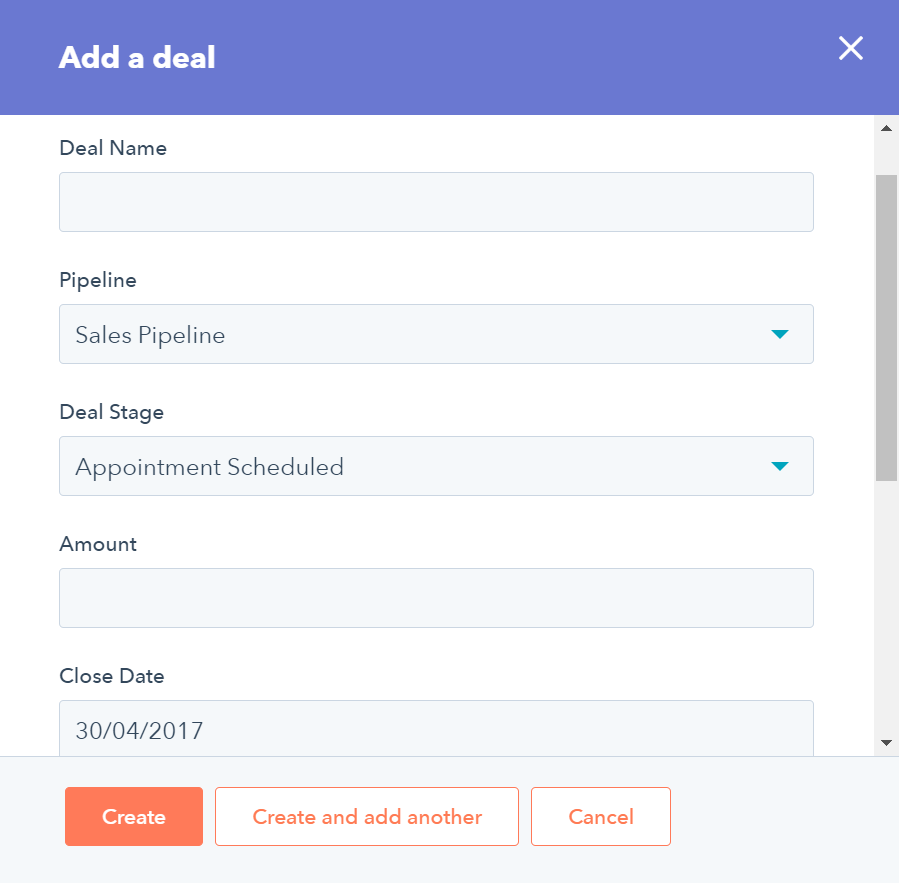
\includegraphics[width=0.5\textwidth]{deal_creation.png}
			\caption{Creando un \textit{deal} desde el portal de \hs{}}
			\label{fig:create_deal}
		\end{figure}

\subsection{Descripción del objeto \textit{Company}}
		
		Es un objeto de \hs{} que representa cualquier tipo de organización o empresa. 
		Este objeto cuenta con multitud de propiedades, que describen información de la empresa, como puede ser información de contacto, localización\ldots 
		
		Desde el portal de \hs{} es posible tanto crear nuevas \textit{companies} como modificar cualquiera de las ya existentes. Podemos ver el formulario de creación de una \textit{company} en la Figura \ref{fig:company_creation}.
		
		Sin embargo la creación o modificación de \textit{companies} no iniciarán procesos de sincronización. Solo se integrarán aquellas \textit{companies} que estén asociadas a un \textit{deal}.
		de esta forma evitamos que \textit{companies} con las que no existe un proyecto estén sincronizadas.
		
		\begin{figure}
			\centering
			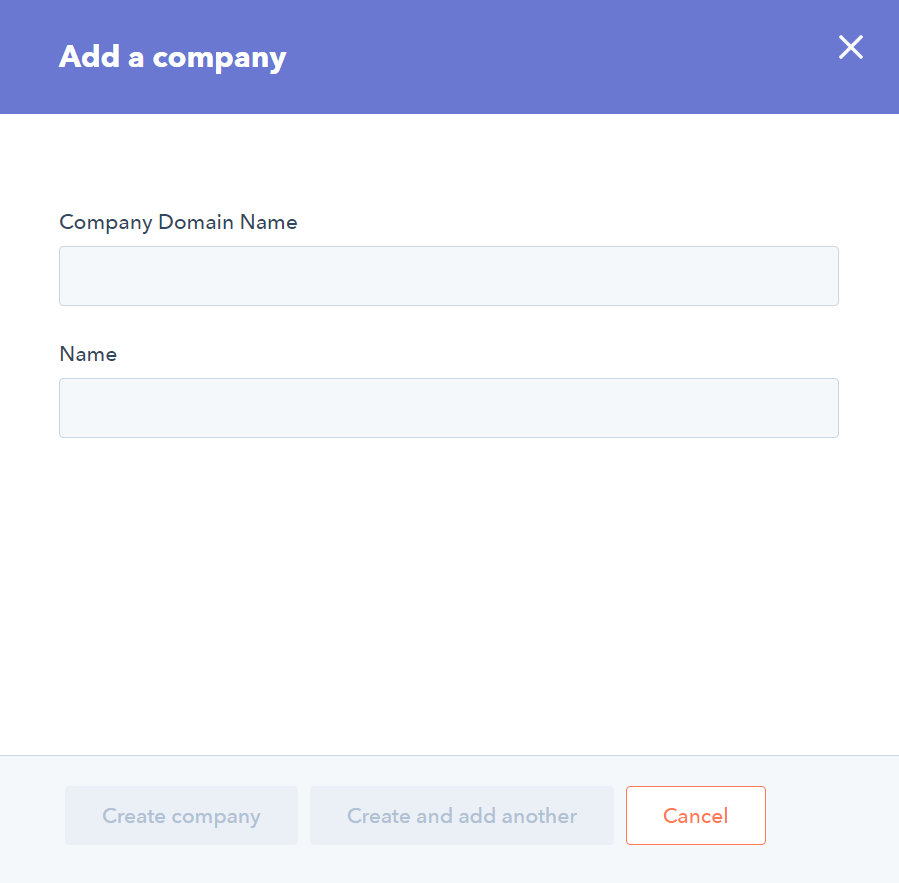
\includegraphics[width=0.5\textwidth]{company_creation.png}
			\caption{Creando una \textit{company} desde el portal de \hs{}}
			\label{fig:company_creation}
		\end{figure}


\subsection{Métodos de integración de \hs{}}
\hs{} cuenta con varios métodos para realizar las integraciones. Cada uno de ellos pensado para distintas situaciones.

\subsubsection{Integración con \textit{API keys}}

Para utilizar este método simplemente hay que consultar la clave de la \acrshort{api} de \hs{} (\textit{HAPIKey}), 
accesible desde el portal de \hs{} y añadirla como parámetro en las peticiones que enviemos al servicio \acrshort{rest} de \hs{}.\\

Este método es idóneo para realizar pruebas. Sin embargo su falta de seguridad impide su uso comercial. %Con este método no se puede garantizar la seguridad.

Además con este método solo es posible la comunicación en un sentido, desde la \iface{} hacia \hs{}.

\subsubsection{Integración con \textit{OAuth}}
\label{subsec:app_hs}

Para poder usar este método de integración es necesario crearse una cuenta de desarrollador. Con la cuenta de desarrollador podemos crear una \textbf{aplicación de \hs{}} y acceder a su panel de control. 

Desde el panel de control podemos ver toda la información de la aplicación. La información que necesitaremos es el identificador de la aplicación, la clave \texttt{Client Id} y la clave \texttt{Client Secret}.

Otra funcionalidad del panel de control es la posibilidad de configurar las suscripciones \textit{Webhook} de \hs{}, que permiten enviar de mensajes desde \hs{} a destinos externos cuando ciertos eventos ocurren.

También podemos hacer un seguimiento del funcionamiento de la aplicación desde el panel de control. \\

Lo primero que necesitamos es instalar la aplicación en el portal de \hs{}.

Para instalar la aplicación en el portal de \hs{} hay que seguir un proceso de autorización llamado \gls{oauth2}. Este proceso se ha automatizado e integrado en la \iface{} creada. 
Los pasos que hay que seguir son los siguientes \cite{hsapi}:
%JSON enviado por el webhook

\begin{enumerate}
	\item Dirigirse a la url de autorización \footnote{\url{https://app.hubspot.com/oauth/authorize?client_id=<client_id>&scope=contacts&redirect_uri=https://www.hubspot.com/} sustituyendo \texttt{<client\_id>} por el su valor}.
	Iniciar sesión en el portal de \hs{} y así autorizar la instalación de la aplicación. Cabe destacar que solo se puede acceder a dicha \textit{url} y por tanto instalar la aplicación si se cuenta con el \texttt{Client ID}. también se necesita un usuario del portal con permisos para poder instalar aplicaciones.
	Haciendo público el \texttt{Client ID} de la aplicación, esta puede ser instalada por cualquier persona en portales a los que tengan acceso. En nuestro caso este valor permanecerá en privado y solo nosotros haremos uso de la aplicación.
		
	\item Tras dar acceso al portal se te redirige a una página en la que aparece como parámetro de la \textit{url} un código.
	\item Mediante este código, el \texttt{Client ID} y el \texttt{Client secret} podemos obtener un token de sesión con una llamada a la \acrshort{api}.
	Tras hacer la petición a la \acrshort{api} de \hs{}, nos devolverá un mensaje \acrshort{json} con los siguientes valores.
		\begin{itemize}
			\item \texttt{access\_token} clave para realizar las peticiones a la \acrshort{api} de \hs{}.
			\item \texttt{refresh\_token} clave para conseguir nuevo par (\texttt{access\_token}, \texttt{refresh\_token}) cuando el \texttt{access\_token} ha expirado.
			\item \texttt{expires\_in} tiempo en milisegundos de validez del \texttt{access\_token}, por defecto son seis horas.
		\end{itemize}
	\item Cuando el \texttt{access\_token} haya expirado podremos llamar a otro \textit{end point} especificando el \texttt{refresh\_token} y recibiremos un mensaje de vuelta con otro nuevo \texttt{access\_token} y \texttt{refresh\_token}.
\end{enumerate}

Usando un \textit{token} válido podremos realizar peticiones a los distintos \textit{endpoint} \acrshort{rest} de \hs{}, es decir, la comunicación de la \iface{} a \hs{}.

Con este método se garantiza que los \textit{token} van variando como mínimo cada seis horas a diferencia del método de integración con \textit{API keys} en el que la  clave es fija y solo varía si lo hacemos manualmente. 

La aplicación instalada sirve como paso intermedio para las comunicaciones entre \hs{} y la \iface{}.

La comunicación en el otro sentido, de \hs{} hacia la \iface{} se hace gracias a la configuración de los \textit{webhook} de \hs{}.

Desde el portal podemos configurar las suscripciónes a los \textit{webhook}. Es necesario especificar la dirección (\textit{host} y puerto) donde deseamos que los mensajes sean enviados ante los diferentes eventos.\\

En el caso de nuestra aplicación está suscrita a los siguientes eventos:
\begin{itemize}
	\item \textbf{deal.creation}: Cuando un nuevo \textit{deal} es creado en \hs{} se envía un mensaje.
	\item \textbf{deal.propertyChanged} 
		\begin{itemize}
			\item \texttt{dealstage}: Cuando en un \textit{deal} de \hs{} se modifica el estado.
			\item \texttt{practice}: Cuando en un \textit{deal} de \hs{} se modifica la práctica.
			\item \texttt{hubspot\_owner\_id}: Cuando en un \textit{deal} de \hs{} se modifica su propietario.
			\item \texttt{closedate}: Cuando en un \textit{deal} de \hs{} se modifica la fecha de cierre.
			\item \texttt{description}: Cuando en un \textit{deal} de \hs{} se modifica la descripción.
			\item \texttt{dealname}: Cuando en un \textit{deal} de \hs{} se modifica el nombre.
			\item \texttt{transaction\_currency}: Cuando en un \textit{deal} de \hs{} se modifica la moneda.
			\item \texttt{legal\_entity}: Cuando en un \textit{deal} de \hs{} se modifica la entidad.
		\end{itemize}
\end{itemize}

La versión que se debe usar de \textit{OAuth} es \textit{OAuth2.0} ya que \hs{} en un futuro no dará soporte a las integraciones con \textit{OAuth1.0}.


\section{\wday{}}

En esta sección vamos a describir la información que necesitamos saber sobre \wday.

\wday{} es un \acrshort{erp} que internamente se encuentra organizado en objetos.
 
Los objetos que van a ser de interés para realizar la integración son:
\textit{Project}, \textit{Customer} y \textit{Hierarchy}.\\

Además cada uno de estos objetos cuenta con una serie de campos, que pueden incluso hacer referencia a otros objetos.
Un \textit{project} tiene un \textit{customer} puede tener asociado y también puede tener dos \textit{hierarchies} asociadas, una opcional y una principal.\\


Para realizar las integraciones, \wday{} proporciona un catálogo de servicios web basados en \acrshort{soap} (\textit{Workday Web Services} \cite{wws}). 
Mediante estos servicios podemos hacer que la \iface{} interactúe con \wday{}.

Cada servicio cuenta con un conjunto de operaciones que pueden ser llamadas mediante su \textit{end point}.\\


Lo siguiente que necesitamos saber es el formato de los mensajes que se deben enviar a estos \textit{end point}. Para ello contamos con el fichero \acrshort{wsdl} de cada servicio que especifica el formato de los mensajes \acrshort{soap} que se deben enviar para realizar cada operación.


El envío de los mensajes se realiza por \acrshort{http}.\\

Una herramienta que se ha utilizado para probar los servicio es \textit{SOAP UI}.

Además es necesario proporcionar credenciales en el mensaje para que \wday{} realice las operaciones deseadas.

Ante estas solicitudes \wday{} siempre responde indicando si la operación se ha realizado correctamente o el error que ha sucedido.



\subsection{Descripción del objeto \textit{Project} en \wday{}}
Es un objeto de \wday{} y existe una instancia por cada proyecto. Dentro de nuestra integración, 
el objeto \textit{Project} de \wday{} se corresponde con el objeto \textit{Deal} de \hs{}. 
De forma que por lo general las acciones sobre el objeto \textit{Deal} en \hs{} darán lugar a otros eventos
 sobre el objeto \textit{Project} de \wday{}.\\
 
Un objeto \textit{Project} puede ser creado de manera manual, pero en nuestra integración, esto se realizará mediante los servicios web.
Para crear o modificar un proyecto ya existente hay que enviar un mensaje \acrshort{soap} por \acrshort{http}. 
Para ello hay que usar la operación \texttt{Submit\_Project}  incluida en el servicio \texttt{Resource\_Management}.\\

El objeto \textit{Project} cuenta con multitud de campos, son de especial importancia los siguientes: 

\begin{itemize}
\item \textbf{\textit{Project name}}: Nombre del proyecto, está sincronizado con el nombre del \textit{deal} correspondiente.
\item \textbf{\textit{Start Date}}: Fecha de inicio, está sincronizado con con la propiedad \texttt{close\_date} del deal.
\item \textbf{\textit{Status}}: Estado del proyecto, existe una correspondencia con la propiedad \texttt{deal\_stage} del deal en \hs{}.
\item \textbf{\textit{Description}}: Descripción del proyecto. Este campo se encuentra sincronizado con la propiedad \texttt{description} del \textit{deal}.
\end{itemize}

Otros campos que hacen referencia a objetos son estos: 
\begin{itemize}
\item \textbf{\textit{Project Hierarchy}}: La Jerarquía principal del proyecto. Este campo está en directa relación con la propiedad personalizadas
\texttt{practice} de \hs.
\item \textbf{\textit{OptionalProject Hierarchy}}: La jerarquía opcional del proyecto. Este campo se encuentra directamente relacionado con la propiedad \texttt{hubspot\_owner\_id} del correspondiente \textit{deal}.
\item \textbf{\textit{Customer}}: El cliente del proyecto. Existe una correspondencia entre el cliente y la asociación \texttt{associated\_company} del \textit{deal} en \hs{}.

\end{itemize}



\subsection{Descripción del objeto \textit{Customer} en \wday{}}
Se trata de un objeto de \wday{} que representa a los clientes de la empresa. este objeto de \wday{} se encuentra relacionado con el objeto \textit{company} de \hs. 
Gracias a la \iface{}, cuando se realice la integración de un \textit{deal}, también se integrará la \textit{company} asociada.\\

Existen múltiples métodos para crear o modificar un \textit{Customer} en \wday{}, de forma manual, hojas de calculo para carga de datos \ldots

En nuestro caso la creación y modificación de un cliente se hace desde la \iface{}, 
mediante la operación \texttt{Put\_Customer} del servicio web \texttt{Revenue\_Management}.

\subsection{Descripción del objeto \textit{Hierarchy} en \wday{}}

El objeto \textit{Hierarchy} de \wday{} se encarga de representar jerarquías.
Es decir, representa información que se encuentra estructurada en forma de árbol.\\

En nuestro caso tenemos una jerarquía principal que organiza los proyectos según a que práctica pertenecen. 
(En el caso de nuestra empresa las distintas prácticas son: \textit{PeopleSoft}, \textit{SAP}, \textit{Cloud} \ldots).\\

También existen jerarquías opcionales para organizar los proyectos según su \textit{Customer Manager} y su \textit{Project Manager}.

\subsection{Servicios web de \wday{}}

Para hacer uso de los servicios web de \wday{}, primero debemos de contar con una cuenta del \textit{tenant} (o entorno) con permisos para el uso de los servicios web que se vayan a usar.

Una vez tengamos dicho usuario, podremos realizar las operaciones.\\

Los pasos para realizar una operación concreta son los siguientes:

\begin{enumerate}
	\item Determinar en que servicio se encuentra la operación deseada.
	\item Conseguir el archivo \acrshort{wsdl}. En este archivo podremos encontrar el formato de mensaje correcto para cada una de las operaciones disponibles en dicho servicio.
	\item Modificar la plantilla de mensaje con los parámetros deseados. 
	Para comprobar que el mensaje realiza la operación deseada correctamente podemos usar la aplicación \textit{SoapUI} \footnote{\url{https://www.soapui.org/}}. %\cite{soapui}.
	\textit{SoapUI} permite abrir esquemas \acrshort{wsdl}, modificar directamente la plantilla del mensaje para cualquier operación del servicio y enviar el mensaje.
	\item Enviar el mensaje \acrshort{soap} por \acrshort{http} con el método POST.
	\item comprobar que no ha habido errores con el mensaje de respuesta proporcionado por \wday.
\end{enumerate}

Para el tratamiento de los mensajes \acrshort{soap} se ha realizado del siguiente modo.
Se ha usado la libreria de \textit{python} \textit{lxml} \footnote{\url{http://lxml.de/}}. 
\begin{enumerate}
	\item Se genera el archivo \textit{xml} con ayuda de la librería \textit{lxml}. Este \textit{xml} cuanta con los parametros necesarios para la llamada al servicio web de \wday{}.
	
	\item Con el archivo \acrshort{xslt} correspondiente se transforma el \acrshort{xml} en el mensaje \acrshort{soap}.
\end{enumerate}

Cuando \wday{} responde con un mensaje \acrshort{soap}, la \iface{} recupera los valores del \acrshort{xml} con ayuda de la librería \textit{lxml}.

\section{\iface{}}


Para el desarrollo de la \iface{} he usado el lenguaje de programación \textbf{python}, con el \textit{IDE} \textbf{PyCharm}. La librería principal, bajo la que se sustenta el servidor es \textbf{\textit{web.py}}.
Alternativas a esta librería pueden ser los \textit{frameworks} \textit{Flask} o \textit{Django}.
\textit{Flask} es un \textit{microframework}, sería una buena alternativa si hubiese que elegir algo distinto a  \textbf{\textit{web.py}}.

\textit{Django} es idónea para proyectos mucho más grandes. Requiera de un proceso más avanzado antes de poder empezar a desarrollar la aplicación.

La ventaja de \textit{web.py} es lo ligera que es y la facilidad de ponerla en marcha.\\

La \iface{} se encuentra ejecutándose de manera continua en un servidor de \textit{amazon} y está escuchando en un puerto los distintos mensajes que puedan llegar de \hs{}.
En el panel de control de la aplicación de \hs{}, explicado en la sección \ref{subsec:app_hs}, debemos especificar el \textit{host} y puerto del servidor que está ejecutando la \iface{}\\


En esta sección vamos a explicar detalladamente el funcionamiento de la \iface{}.

\subsection{Estructura de la \iface{}}
Vamos a describir como se encuentra estructurada nuestra \iface. Para ello podemos ver la Figura \ref{fig:project_structure}. 

El proyecto de \textit{python} se encuentra organizado en diferentes archivos subdirectorios.

\begin{itemize}

	\item [\textendash] \textbf{\textit{service.py}}: Se encuentra en el directorio raíz y se encarga de ejecutar la aplicación 
	y en este modulo está definida la función que se ejecuta al recibir un mensaje \textit{POST}. Desde este módulo se hacen llamadas a distintas funciones de \textit{handler.py}.
	\item [\textendash] \textbf{\textit{handler.py}}: También se encuentra en el directorio raíz y en este módulo se encuentra la lógica de programa para cada evento recibido.
	\item[\textendash] \textbf{\textit{hubspot}}: En este directorio se encuentran todos los módulos de \textit{python} que implementan funcionalidades para interactuar con \hs.
	
		\begin{itemize}
			\item [\textendash] \textbf{\textit{deal.py}}: En este módulo se encuentra la clase \textit{Deal}, encargada de representar en la \iface{} el objeto \textit{deal} de \hs.
			\item [\textendash] \textbf{\textit{company.py}}: En este módulo se encuentra la clase \textit{Company}, que se encarga de representar al objeto \textit{company} de \hs{}.
			\item [\textendash] \textbf{\textit{authorization.py}}: En este módulo se encuentra la clase Authorization encargada de facilitar el flujo de aprobación \gls{oauth2} de \hs{} y la renovación de los \textit{token} de sesión.
		\end{itemize}
		
	\item[\textendash] \textbf{workday}: En este directorio están los módulos encargados de la interacción con \wday.
	
		\begin{itemize}
			\item [\textendash] \textbf{\textit{project.py}}: En este módulo se encuentra la clase \textit{Project} que representa en la \iface{} el objeto \textit{Project} de \wday.
			\item [\textendash] \textbf{\textit{custommer.py}}: En este módulo se encuentra la clase \textit{Customer} que representa en la \iface{} el objeto \textit{Customer} de \wday.
			\item [\textendash] \textbf{\textit{hierarchy.py}}: En este módulo se encuentra la clase \textit{Hierarchy} que representa en la \iface{} el objeto \textit{Hierarchy} de \wday.
		\end{itemize}
	\item[\textendash] \textbf{modules}: En este directorio se encuentran agrupados módulos con funcionalidades diversas. 
	
			\begin{itemize}
				\item [\textendash] \textbf{\textit{configuration.py}}: En este módulo es donde inicializamos los \textit{Parser} de cada uno de los archivos de configuración.
				\item [\textendash] \textbf{\textit{database.py}}: Módulo para inicializar de las tablas de la base de datos y para la realización de operaciones en estas tablas.
				\item [\textendash] \textbf{\textit{log.py}}: Módulo encargado de implementar la salida a ficheros registro.
				\item [\textendash] \textbf{\textit{mail.py}}: Este módulo se encarga de la funcionalidad necesaria para enviar \textit{emails}.
			\end{itemize}
			
	\item[\textendash] \textbf{cfg}: En este directorio se encuentran todos los archivos de configuración. 
	Por lo general permanecen invariantes. A excepción de aquellos que almacenan \textit{tokens} de sesión que van cambiando.
	\item[\textendash] \textbf{xslt}: En este directorio se encuentran todas las plantillas de transformación necesarias para enviar los mensajes a \wday.
	Partiendo de un archivo \acrshort{xml}, podemos transformarlo con estas plantillas y generar un mensaje \acrshort{soap} para su posterior envío a \wday.
	

\end{itemize}

\begin{figure}
\centering
\tikzstyle{every node}=[draw=black,thick,anchor=west]
\tikzstyle{python}=[draw=blue,very thick, fill=blue!10, rounded corners]
\tikzstyle{folder}=[draw=orange,very thick,fill=orange!10]
%\tikzstyle{cfg}=[draw=red,fill=gray!50]
%\tikzstyle{xslt}=[draw=red,fill=gray!50]
\begin{tikzpicture}[
	scale=0.9,
  grow via three points={one child at (0.5,-1) and
  two children at (0.5,-1) and (0.5,-2)},
  edge from parent path={(\tikzparentnode.south) |- (\tikzchildnode.west)}]
	
	\node [folder]{ \Large Interfaz}
    child { node [python]{service.py}}		
    child { node [python]{handler.py}}
    child { node [folder] {hubspot}
      child { node [python]{deal.py}}
      child { node [python]{company.py}}
      child { node [python]{authorization.py}}
    }
	child [missing] {}				
    child [missing] {}				
    child [missing] {}
	child { node [folder] {workday}
      child { node [python]{project.py}}
      child { node [python]{customer.py}}
      child { node [python]{hierarchy.py}}
    }
	child [missing] {}				
    child [missing] {}				
    child [missing] {}
	child { node [folder] {modules}
      child { node [python]{configuration.py}}
      child { node [python]{database.py}}
      child { node [python]{log.py}}
	  child { node [python]{mail.py}}
    }
	child [missing] {}				
    child [missing] {}				
    child [missing] {}
	child [missing] {}				
	child { node [folder] {cfg}}
	child { node [folder] {xslt}};
	
	
	
\end{tikzpicture}
\caption{Estructura de la interfaz} \label{fig:project_structure}
\end{figure}


\subsection{Almacenamiento persistente}

En la \iface{} existen dos tipos de almacenamiento persistente: Estático y dinámico.

\begin{itemize}[leftmargin=*]
\item \textbf{Estático}: Se trata de los archivos de configuración ubicados en el directorio \textit{cfg} que se pueden ver en la Figura \ref{fig:project_structure}.
En estos archivos se guarda información como usuarios, contraseñas, \textit{token} de sesión, direcciones \textit{url}\ldots
De esta forma se evita que estos datos se encuentren escritos directamente en el código como constantes. Nos facilita su modificación e
incluso la posibilidad de excluirlos fácilmente cuando se añada el proyecto a repositorios públicos.
Está información es fija (a excepción de los \textit{token} de sesión). Solo se cambiará cuando sea necesaria otra configuración.\\

Para su implementación he usado el módulo \textit{ConfigParser} \footnote{\url{https://docs.python.org/2/library/configparser.html}} parte de una librería estandar. \textit{ConfigParser} facilita la lectura de archivos de configuración. A estos archivos se les suele poner la extensión \textit{ini}. %TODO footnote cofigparser
Estos archivos de configuración se organizan en secciones formadas por listas de parejas clave-valor.
Una ventaja al usar \textit{ConfigParser} es que a la hora de definir una pareja clave-valor se puede referenciar un valor definido en la sección \textit{DEFAULT}. 


Otras alternativas para los archivos de configuración son \textit{yaml}, \textit{xml}, \textit{json}\ldots


\begin{itemize}
	\item [\textendash] \textbf{\textit{hubspot.ini}}: En este archivo se guarda la información referente a los \textit{tokens} de sesión, necesarios para comunicarse con el portal de \hs. 
	Este archivo cambia cada vez que se actualiza un \textit{token}.
	\item [\textendash] \textbf{\textit{workday.ini}}: En este archivo de configuración se 
	guardan las credenciales de acceso a \wday{}, así como distintas direcciones url para evitar su repetición en el código.
	\item [\textendash] \textbf{\textit{mapping.ini}}: En este archivo de configuración se encuentran todas las correspondencias entre \hs{} y \wday.
	\item [\textendash] \textbf{\textit{mail.ini}}: En este archivo de configuración se encuentran las credenciales necesarias para el acceso a la cuenta de correo.
\end{itemize}




\item \textbf{Dinámico}: Se trata de la base de datos local \textit{SQLite3} \footnote{\url{https://docs.python.org/2/library/sqlite3.html}} para \textit{python}. %TODO footnote sqlite3
 En esta base de datos se almacenan las distintas correspondencias entre \hs{} y \wday.
 
 Existen tres tablas en la base de datos: \texttt{deals\_excluded}, \texttt{deal\_project} y \texttt{company\_customer}.
 
 
 \begin{itemize}
	\item \texttt{deals\_excluded}: En esta tabla se almacena los identificadores de los \textit{deals} de \hs{} 
	que se encuentran excluidos para la integración. Todos los \textit{deals} que se encuentren en la fase de
	cierre estarán excluidos.
	\item \texttt{deal\_project}: En esta tabla se encuentra la correspondencias entre identificadores 
	de \textit{deals} de \hs{} y los identificadores de los \textit{projects} en \wday{}, para todos los \textit{deals} que han sido integrados.
	\item \texttt{company\_customer}: En esta tabla se encuentra la correspondencia entre las \textit{company} de \hs{} y los \textit{customers} de \wday{}
	para todos los \textit{companies} que hayan sido integrados.
 \end{itemize}
 

\begin{table}[H]
		\centering
		\begin{tabular}{
		|c|c@{\hskip 1cm} 
		|c|c|c@{\hskip 1cm} 
		|c|c|c@{\hskip 1cm}
		}
		\cline{1-1}\cline{3-4}\cline{6-7}
		deals\_excluded && \multicolumn{2}{c|}{deals\_excluded} && \multicolumn{2}{c|}{company\_customer} \\
	\cline{1-1}\cline{3-4}\cline{6-7}
	deal id && deal id & project id && company id & customer id \\
	\cline{1-1}\cline{3-4}\cline{6-7}
	\end{tabular}
	\caption{Tablas en la base de datos local}
	\label{tab:tables}
\end{table}

\end{itemize}




\subsection{Seguridad}
\label{subsec:security}

La \iface{} se encuentra escuchando los mensajes que le son enviados. Pero ¿Cómo podemos garantizar que el mensaje que recibimos proviene realmente de \hs{}?
Para ello existe un campo en la cabecera del mensaje recibido, que es \texttt{HUBSPOT\_SIGNATURE}. 
Este campo es el formado tras aplicar la función \textit{hash \textbf{sha256}} a la concatenación del \texttt{Client Secret} de nuestra aplicación de \hs{} con el cuerpo del mensaje \acrshort{http} recibido.\\

Basta hacer esta comprobación para garantizar la procedencia del mensaje, ya que el \texttt{Client Secret} solo es conocido por nosotros y por \hs{}. \\

Además cabe destacar que cualquier persona que interceptase el mensaje, no podría deducir el \texttt{Client Secret}, gracias a las propiedades de las funciones \textit{hash}. 

%TODO cite function hash


% A hash function is any function that can be used to map data of arbitrary size to data of fixed size. The values returned by a hash function are called hash values, hash codes, digests, or simply hashes. One use is a data structure called a hash table, widely used in computer software for rapid data lookup. Hash functions accelerate table or database lookup by detecting duplicated records in a large file. An example is finding similar stretches in DNA sequences. They are also useful in cryptography. A cryptographic hash function allows one to easily verify that some input data maps to a given hash value, but if the input data is unknown, it is deliberately difficult to reconstruct it (or equivalent alternatives) by knowing the stored hash value. This is used for assuring integrity of transmitted data, and is the building block for HMACs, which provide message authentication.

Como podemos comprobar en la Figura \ref{fig:validation_message}, aquellos mensajes que no cumplen los requisitos, se ignoran. Esto protege a nuestra \iface{} de aquellos mensajes no autorizados.

\begin{figure}
\centering

\shorthandoff{'}



\tikzstyle{line} = [draw, -latex']
\tikzstyle{startstop} = [rectangle, rounded corners, minimum width=3cm, minimum height=1cm,text centered, draw=black, fill=red!30]
\tikzstyle{io} = [trapezium, trapezium left angle=70, trapezium right angle=110, minimum width=3cm, minimum height=1cm, text centered, draw=black, fill=blue!30]
\tikzstyle{process} = [rectangle, minimum width=3cm, minimum height=1cm, text centered, draw=black, fill=orange!30]
\tikzstyle{decision} = [diamond, aspect=2,  minimum width=3cm, minimum height=1cm, text centered, draw=black, fill=green!30]
    
\begin{tikzpicture}[node distance = 3cm, auto]
	
	\node [io] (message) {Mensaje externo};
	\node [decision,below of =message] (valid) {¿Válido?};
	\node [startstop, below right of=valid, xshift=2cm, yshift=1cm] (no_valid) {Se ignora};
	\node [decision,below of =valid] (tipo) {¿Tipo?};
	
	\node [process, below left of=tipo, xshift=-2cm] (deal_creation) {Crear deal};
	\node [process, below right of=tipo, xshift=2cm] (deal_modification) {Modificar deal};
	
	\path [line] (message) -- (valid);
	\path [line] (valid.east) -| node {no}(no_valid);
	\path [line] (valid.south) -- node {sí}(tipo);
	
	\path [line] (tipo.west) -| node [left] {deal creation}(deal_creation);
	\path [line] (tipo.east) -| node {deal modfication}(deal_modification);
	
	
\end{tikzpicture}



\caption{Validación de los mensajes recibidos por la Interfaz} \label{fig:validation_message}
\end{figure}


\subsection{Flujo del programa}
%Dependiendo de de las acciones realizadas en \hs{}, se puede disparar un evento y que consiguientemente un mensaje se envíe a la \iface.

Como se ha mencionado anteriormente, nuestra aplicación de \hs{} está suscrita a diferentes eventos de los \textit{deals} de \hs{}.
Cuando uno de estos eventos se produce, la aplicación de \hs{} envía un mensaje \acrshort{http} (\textit{POST}) a la \iface{}. Este mensaje es un \acrshort{json} con información sobre el evento ocurrido. Podemos ver un mensaje de ejemplo en el Código \ref{lst:json_message}.\\

Para probar el correcto funcionamiento de la interfaz sin realizar cambio en \hs{}, se ha usado la herramienta \textit{cURL} \footnote{\url{https://curl.haxx.se/}}. 
Con \textit{cURL} podemos simular las peticiones \acrshort{http} enviadas desde \hs{}.

\begin{figure}
\begin{lstlisting}[caption={Ejemplo de mensaje recibido por la \iface{}},label={lst:json_message}, language=json]
	[{"objectId":92604011,
	  "changeFlag":"NEW",
	  "changeSource":"",
	  "eventId":2763628519,
	  "subscriptionId":1794,
	  "portalId":1234,
	  "appId":5678,
	  "occurredAt":1485865855549,
	  "subscriptionType":"deal.creation",
	  "attemptNumber":0}]
\end{lstlisting}
\end{figure}
 
Una vez recibido el mensaje se comprueba su validez verificando su procedencia como hemos visto en la Sección \ref{subsec:security}. Aquellos mensajes inválidos se ignoran como podemos ver en el diagrama de la \ref{fig:validation_message}.\\

Tras verificar que un mensaje es válido, se comprueba si dicho \textit{deal} se encuentra en la tabla de excluidos de base de datos local (\texttt{deals\_excluded}). 
Esta comprobación sirve como precaución para evitar la sincronización de proyectos no deseados en \wday{}.

Después dependiendo del valor del campo \textit{subscriptionType} comienza la ejecución de un proceso de creación de un deal o de modificación.

\begin{itemize}
	\item \textbf{Creación de un \textit{deal}}: Si el valor del atributo \textit{subscriptionType} es \textit{deal.creation}, éste nos indica que un \textit{deal} ha sido creado.
		En el mensaje \acrshort{json} también se especifica el id del \textit{deal} creado (\textit{objectId}) y otros datos de relevancia como el id del portal, id de la aplicación, momento en el que ocurrió el evento\ldots \\
	
		
		Los pasos que se siguen para el procesamiento del mensaje son los siguientes:
		
		\begin{enumerate}
			\item Se comprueba si el \textit{deal} está excluido, si es así entonces la petición no se procesa.
		
			\item Se comprueba si el \textit{deal} tiene una entrada en la tabla de correspondencias entre los \textit{deals} y \textit{projects} (\texttt{deals\_project}).
		En la tabla \texttt{deals\_project} se guarda la correspondencia entre los identificadores de los \textit{deals} de \hs{} y los identificadores de los \textit{projects} de \wday{} que están integrados.
		En caso de que el \textit{deal} esté en la tabla de correspondencias, quiere decir que el \textit{deal} se ha creado previamente y por tanto la petición se ignora y para el proceso.\\
		
		Si por el contrario no se encuentra en la tabla de correspondencias entonces se continua con el siguiente paso.
		
			\item Se realiza una petición a la \acrshort{api} de \hs{} para obtener el resto de información del \textit{deal} creado.
			\item Con todos los datos del \textit{deal} que se ha creado se comprueba si este se encuentra en la fase de progreso, en caso contrario dicho \textit{deal} no se integra y se para el proceso.
			\item Si el \textit{deal} se encuentra en la fase de progreso, entonces se comprueba si el \textit{company} asociado al \textit{deal} existe en la tabla de correspondencias entre los \textit{companies} y los \textit{customers} (\texttt{company\_customer}).
			En caso de que no exista se crea el correspondiente \textit{customer} en \wday{}, y se actualiza la tabla \texttt{company\_customer} con la nueva entrada .
			
			\item Se crea el \textit{project} asociándolo con el \textit{customer} previamente creado o existente y se actualiza la tabla \texttt{deals\_project} con la nueva correspondencia.
		\end{enumerate}
		
		
		
		\begin{figure}
\centering

\shorthandoff{'}



\tikzstyle{line} = [draw, -latex']
\tikzstyle{startstop} = [rectangle, rounded corners, minimum width=3cm, minimum height=1cm,text centered, draw=black, fill=red!30]
\tikzstyle{io} = [trapezium, trapezium left angle=70, trapezium right angle=110, minimum width=3cm, minimum height=1cm, text centered, draw=black, fill=blue!30]
\tikzstyle{process} = [rectangle, minimum width=3cm, minimum height=1cm, text centered, draw=black, fill=orange!30]
\tikzstyle{decision} = [diamond, aspect=2, minimum width=3cm, minimum height=1cm, text centered, draw=black, fill=green!30]
    
\begin{tikzpicture}[node distance = 3cm, auto]
	
	\node [startstop] (deal_creation) {Crear \textit{Deal}};
	\node [decision,below of =deal_creation] (db) {¿Está en BD?};
	\node [startstop, below right of=db, xshift=2cm, yshift=1cm] (in_db) {Se ignora el mensaje};
	\node [process,below of =db] (get_deal) {Obtener \textit{deal} de HubSpot};
	\node [decision,below of =get_deal] (valid) {\begin{tabular}{c}¿\textit{Dealstage} \\ válido? \end{tabular}};
	\node [process, below of=valid] (submit_customer) {Subir \textit{customer} a Workday};
	\node [process, below of=submit_customer] (submit_project) {Subir \textit{project} a Workday};
	
	
	\path [line] (deal_creation) -- (db);
	\path [line] (db.east) -| node {si}(in_db);
	\path [line] (db.south) -- node {no}(get_deal);
	\path [line] (get_deal.south) -- (valid);
	\path [line] (valid.south) -- node [left] {si} (submit_customer);
	\path [line] (valid.east) -| node [right] {no} (in_db);
	\path [line] (submit_customer.south) -- (submit_project);
	
	
\end{tikzpicture}



\caption{Proceso Crear Deal} \label{fig:deal_creation}
\end{figure}
		
		
	\item \textbf{Modificación de un \textit{deal}}:
	
		Si atributo \textit{subscriptionType} en el mensaje \acrshort{json} recibido tiene el valor \textit{deal.propertyChange}, quiere decir que se ha producido el cambio de alguna propiedad en un \textit{deal} de \hs{}.
		
		Los pasos que se siguen ante este tipo de mensajes son los siguientes:
		
		\begin{enumerate}
			\item Se comprueba si dicho \textit{deal} se encuentra en la tabla \texttt{deals\_excluded} de base de datos local. En tal caso, se para el proceso y no se sincronizan las modificaciones en \wday{}.
			\item Se comprueba si el \textit{deal} existe en la tabla de correspondencias \texttt{deal\_project}. De no ser así se procede a la creación del \textit{deal} con el proceso detallado anteriormente.
			\item Se obtiene el objeto \textit{project} de \wday{}. Se actualizan los correspondientes campos localmente, dependiendo de la propiedad del \textit{deal} que haya cambiado. Por último se actualiza el objeto \textit{project} correspondiente de \wday{} con los cambios realizados.
		\end{enumerate}
		
		
		
		Cuando un \textit{deal} pasa a un estado perteneciente a la fase de cierre, el \textit{deal} se añade a la tabla de excluidos \texttt{deals\_excluded}.
		
		
		\begin{figure}[H]
\centering

\shorthandoff{'}



\tikzstyle{line} = [draw, -latex']
\tikzstyle{startstop} = [rectangle, rounded corners, minimum width=3cm, minimum height=1cm,text centered, draw=black, fill=red!30]
\tikzstyle{io} = [trapezium, trapezium left angle=70, trapezium right angle=110, minimum width=3cm, minimum height=1cm, text centered, draw=black, fill=blue!30]
\tikzstyle{process} = [rectangle, minimum width=3cm, minimum height=1cm, text centered, draw=black, fill=orange!30]
\tikzstyle{decision} = [diamond, aspect=2, minimum width=3cm, minimum height=1cm, text centered, draw=black, fill=green!30]
    
\begin{tikzpicture}[node distance = 3cm, auto]
	
	\node [startstop] (deal_modification) {Modificar Deal};
	\node [decision,below of =deal_modification] (db) {¿Está en BD?};
	\node [process, below right of=db, xshift=2cm, yshift=1cm] (not_in_db) {Crear Deal};
	\node [process,below of =db] (get_deal) {Obtener deal de HubSpot};
	\node [process, below of=get_deal] (update_project) {Subir project en Workday};
	
	
	\path [line] (deal_modification) -- (db);
	\path [line] (db.east) -| node {no}(not_in_db);
	\path [line] (db.south) -- node {si}(get_deal);
	\path [line] (get_deal.south) -- (update_project);
	
	
\end{tikzpicture}



\caption{Proceso Modificar Deal} \label{fig:deal_modification}
\end{figure}

\end{itemize}



